\documentclass[tikz,border=10pt]{standalone}
%\usepackage[T1]{fontenc}
\usepackage[utf8]{inputenc}

\usepackage{amsmath}
\usepackage{amsfonts}
\usepackage{amssymb}
\usepackage{mathtools}

\usepackage{graphics}

\usepackage{tikz}
\usetikzlibrary{calc}
\usetikzlibrary{arrows}
\usetikzlibrary{positioning}

\definecolor{light-gray}{gray}{0.95}

\begin{document}
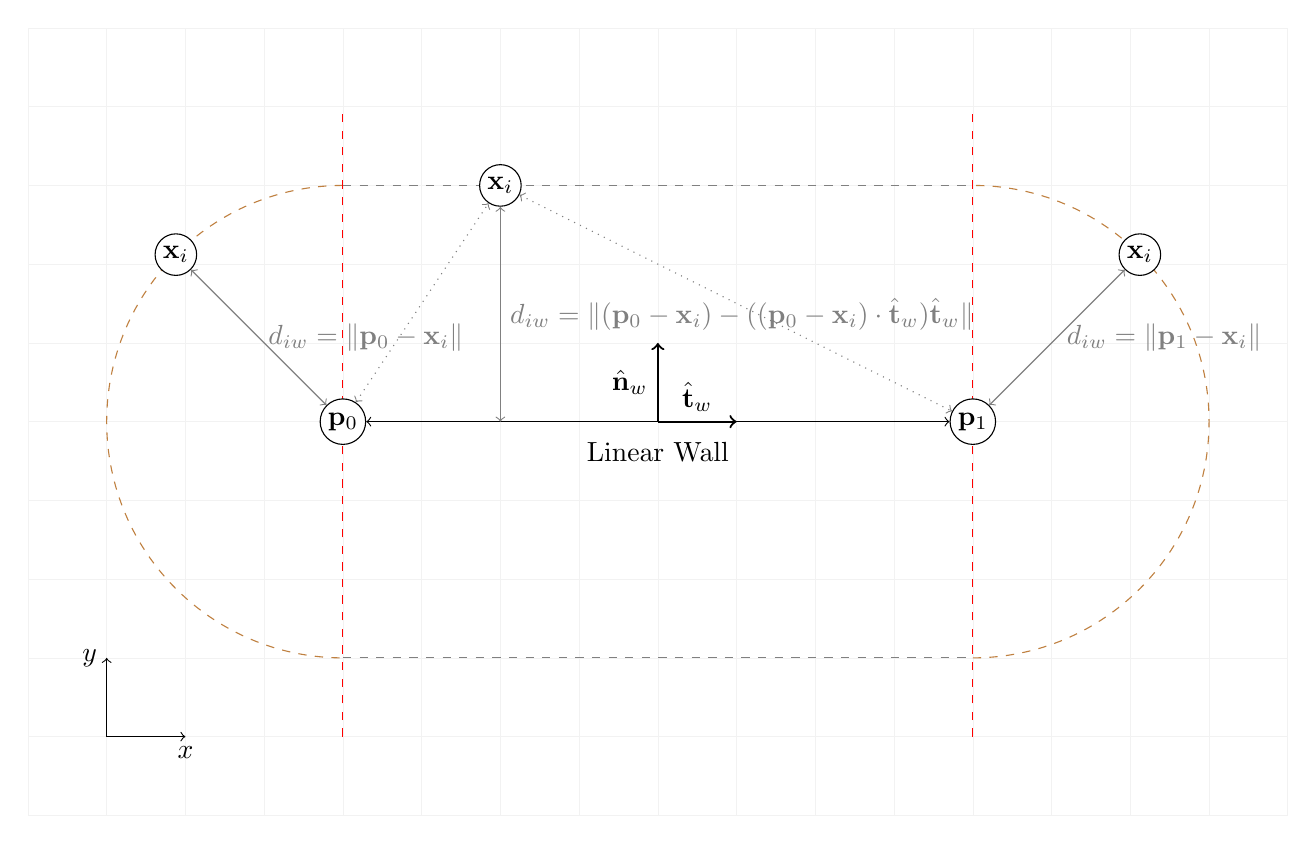
\begin{tikzpicture}
  [
    point/.style = {draw, circle, fill=white, inner sep=1.4pt}
  ]
% Grid (x, y)
\coordinate[] (p1) at (-8, -5);
\coordinate[] (p2) at ( 8,  5);
\draw[help lines, step=1, light-gray] (p1) grid (p2);

\coordinate[] (xp) at ($ (p1) + (1, 0) + (1, 1) $);
\coordinate[] (yp) at ($ (p1) + (0, 1) + (1, 1) $);
\node[anchor=north] (x) at (xp)  {$ x $};
\node[anchor=east] (y) at (yp) {$ y $};
\draw[<->] (xp) -- ($ (p1) + (1, 1) $) -- (yp);

% ---------------------------------------------------
% Start - End - Mid - nodes
\coordinate[] (p0) at  (-4, 0);
\coordinate[] (p1) at  ( 4, 0);
\coordinate[] (off) at ( 0, 3);

% Vertical Lines
\draw[dashed, gray] ($ (p0) + (off) $) -- ($ (p1) + (off) $);
\draw[dashed, gray] ($ (p0) - (off) $) -- ($ (p1) - (off) $);
% Arcs
\draw[dashed, brown] ($ (p0) + (off) $) arc (90:270:3);
\draw[dashed, brown] ($ (p1) - (off) $) arc (-90:90:3);
% Horizontal Line - Separator
\draw[dashed, red] ($ (p0) - (off) - (0, 1) $) -- ($ (p0) + (off) + (0, 1) $);
\draw[dashed, red] ($ (p1) - (off) - (0, 1) $) -- ($ (p1) + (off) + (0, 1) $);
% Linear wall
\node[point] (start) at (p0) {$ \mathbf{p}_{0} $};
\node[point] (end)   at (p1) {$ \mathbf{p}_{1} $};
\coordinate[] (mid) at ($ (p0) + (p1) $);  % / 2
\path[] (start)
        edge[<->] node[below=4pt, midway]{Linear Wall} 
        (end);
% Normal
\path[] (mid)
        edge[->, thick] node[left, midway]{$ \hat{\mathbf{n}}_{w} $} 
        ($ (mid) + (0, 1) $);
% Tangent
\path[] ($ (mid) + (0, 0) $) 
        edge[->, thick] node[above, midway]{$ \hat{\mathbf{t}}_{w} $} 
        ($ (mid) + (1, 0) $);
% Pedestrians
% Inside of red separator lines
% https://en.wikipedia.org/wiki/Distance_from_a_point_to_a_line
\node[point] (x1) at ($ (start) + (2, 3) $) {$ \mathbf{x}_{i} $};
\path[] (start)
        edge[<->, gray, dotted] node[right, midway]{}
        (x1);

\path[] (x1)
        edge[<->, gray, dotted] node[right, midway]{}
        (end);

\path[] (x1)
        edge[<->, gray] node[right, midway]{$ d_{iw} = \| (\mathbf{p}_{0}-\mathbf{x}_{i}) - ((\mathbf{p}_{0}-\mathbf{x}_{i}) \cdot \hat{\mathbf{t}}_{w}) \hat{\mathbf{t}}_{w} \| $}
        ($ (start) + (2, 0) $);
% Left of red separator line
\node[point] (x2) at ($ (start) + ({3 * cos(90+45)}, {3 * sin(90+45)}) $) {$ \mathbf{x}_{i} $};
\path[] (start)
        edge[<->, gray] node[right, midway]{$ d_{iw} = \left\| \mathbf{p}_{0}-\mathbf{x}_{i} \right\| $}
        (x2);
% Right of red separator line
\node[point] (x2) at ($ (end) + ({3 * cos(45)}, {3 * sin(45)}) $) {$ \mathbf{x}_{i} $};
\path[] (end)
        edge[<->, gray] node[right, midway]{$ d_{iw} = \left\| \mathbf{p}_{1}-\mathbf{x}_{i} \right\| $}
        (x2);
% ---------------------------------------------------
\end{tikzpicture}
\end{document}